\chapter{Research Context}
\graphicspath{{Chapter2/Figs/}{Chapter2/Figs/}}

This chapter describes the research question's context and the current literature findings. The reader is educated on neuroscientific limitations, the state of current non-invasive and unidirectional BCIs, the paradigm shift in developing cloud-based and production-ready software and the implications of web-based approaches to BCIs and 3D applications for VR and AR that go hand in hand with BCI technologies.

\section{Limitations of BCIs}
\label{chapter2-limitations-of-bcis}

The possibilities of BCIs are not without limitations. In addition to the hardware limitations, the author attempts to address a broader issue related to neuropsychology that directly correlates with the software aspects, in addition to the challenges of computability.

\subsection{Decoding brain data}
\label{chapter2-decoding-brain-data}

As outlined in the previous chapter, a holistic view of BCI must take into account the aspect of decoding measured neural data and making it intelligible to computer software. It is important to emphasise that the task of decoding neural data is different from decoding thoughts, which is a critical factor for software. Moreover, decoding neural data and extracting the thoughts behind it so that the software can understand them are disciplines on their own. For example, getting computers to recognise letters written on a photograph is a very different problem from reading the written words in the sentences (i.e. computer vision and natural language processing).

Another part is understanding the sentences and their meaning, as in natural language understanding (NLU). NLU is considered an AI-hard problem, which means that the difficulty of these computational problems is equivalent to solving the central problem of artificial general intelligence\footnote{Based on the assumption that general human-level intelligence is computable.} (AGI) \citep{demasi_theoretical_2010}. Understanding less structured data, such as EEG data, is more complicated than understanding structured and human-generated syntax such as written language because it contains more hidden features than a paragraph of text. As a result, the author assumes that understanding brain data might be considered an AI-hard problem.

\subsection{Abstract thoughts}
\label{chapter2-abstract-thoughts}

\begin{figure}[ht]
  \centering
  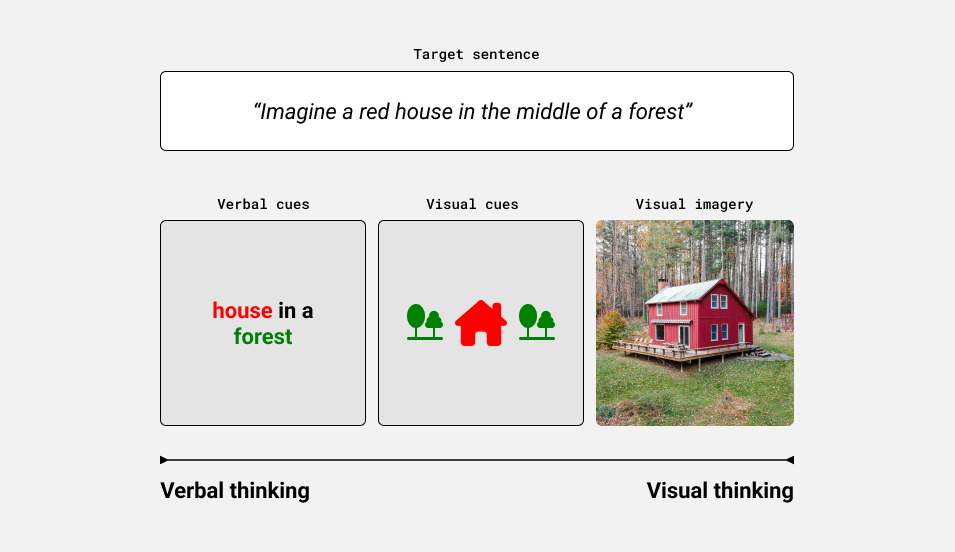
\includegraphics[width=\linewidth]{visual-thinking.png}
  \caption{Difference between verbal and visual thinking using the target sentence of a red house in the middle of a forest (own representation, 2022).}
  \label{fig:visual-thinking}
\end{figure}

Imagine a red house in the middle of a forest. Depending on the individual thought process, one can imagine the house with temporary visual imagery in mind, as in visual thinking, or one can imagine it more verbally, such as conceptually comprehending each word sequentially of what a red house is and that it is located in a forest \citep{amit_asymmetrical_2017}. Additionally, it should also be addressed that different types of thoughts exist at different levels of abstraction and complexity. One can assume that the visual image of a red house in the forest is more abstract and far-fetched than, say, the movement of one's own thumbs, which has a clear physical counterpart. It gets even more complicated when one imagines concepts that are inconceivable to visualise, such as the idea of a company. A company is only an abstract, collectively agreed upon concept without a physical counterpart\footnote{Some people might think of a company building when imaging a company, others might imagine their website, their logo or physical products etc.} and is, therefore, even less straightforward and more complex to decode the meaning of measured brain activity than the other mentioned examples of the red house.

\subsection{Technological limitations}
\label{chapter2-technological-limitations}

\begin{figure}[ht]
  \centering
  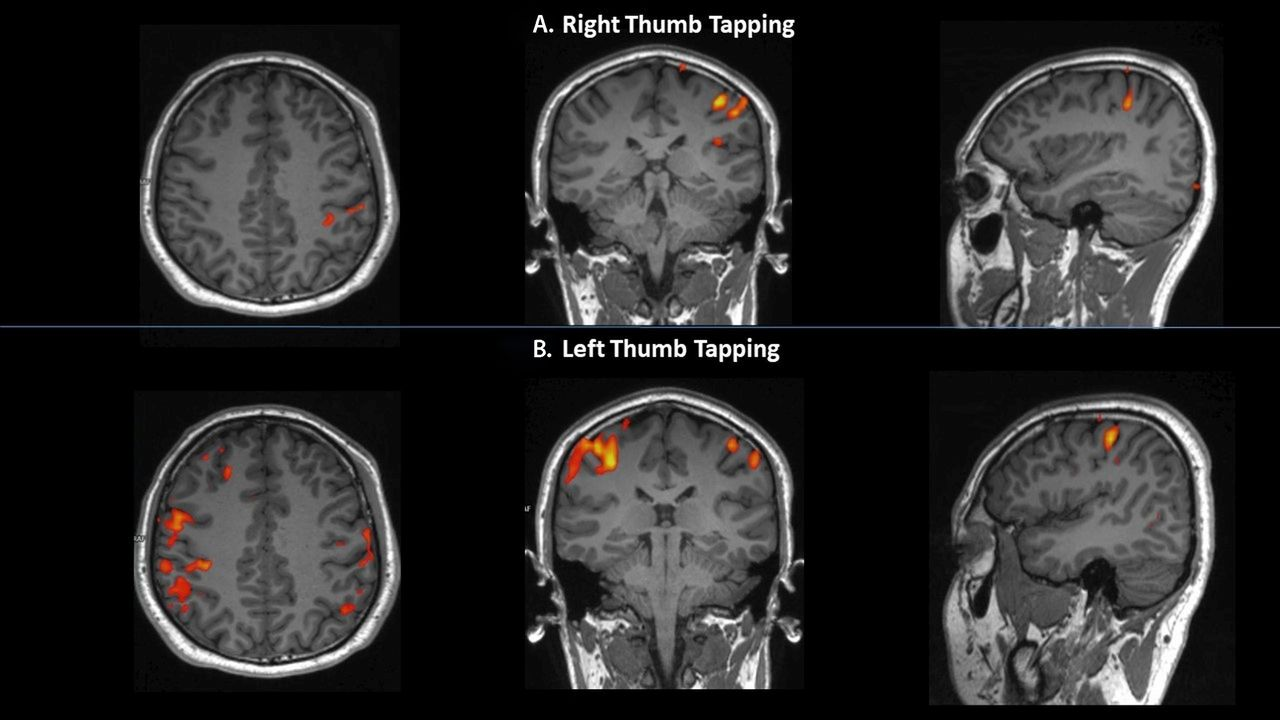
\includegraphics[width=\linewidth]{fmri-scan.jpg}
  \caption{Image of localised activation of neurons during right and left thumb movement using functional magnetic resonance imaging (fMRI) \citep{rashid_bilateral_2018}.}
  \label{fig:fmri-scan}
\end{figure}

Most functional tasks of the brain are localised, which means that these signals are generated by local brain areas that can be identified, such as the motor cortex, which has been shown to be responsible for muscle movement as shown in \autoref{fig:fmri-scan}. Examining the areas of the brain responsible for activating individual muscle strands can yield a comparable response of muscle stimulation in the brain and thus be measured as output for software to move a prosthesis, for example. However, the more specific, less functional, more behavioural and abstract the thoughts are, the less the brain areas are spatially visible. The intent of identifying, for example, the thought of a red house in a forest in verbal thought, the author identified three technological problem statements:

\begin{itemize}
  \item To understand single thoughts, it is essential to have sufficiently clear data from experiments with a certain level of detail (e.g., at the level of detail related to the firing of action potential of individual neurons) as well as temporal precision (an action potential takes about 1 ms to arise) to perform studies to extract possible localisation of individual thoughts. Current neuroimaging technologies cannot capture every process in sufficient detail of the entire brain at once to extract the activity of, e.g. individual neurons while also having high temporal precision.
  \item Even if we could measure every single neuron in the brain with high temporal precision, we would have an extreme amount of data generated concisely. Let us say we would collect a float per neuron that represents the rate of change in voltage with respect to time with a frequency of 1 ms and then record each neuron in the brain a million times a second, taking into account that the average human brain has around 86 billion neurons; we would generate 305.53337637684 petabytes of data per second. This is currently not feasible for commercially available storage and processing resources.
  \item Even if we have the technology, it is a challenge because reproducibility of experiments is very difficult for neuroscientific studies. It is probably impossible to generate clean-slate neural data that is comparable to previously recorded data. Our neurophysiological brain structure changes over time due to neuroplasticity \citep{puderbaugh_neuroplasticity_2022}, and we are in different states of mind every millisecond of our existence, which can have different influences, such as insufficient sleep, something disturbing someone, mental distraction due to an important event that may have occurred since the last measurement, or a salient thought that occurs during a measurement.
\end{itemize}

\subsection{Lack of data}
\label{chapter2-lack-of-data}

As pointed out in the previous section, points 2 and 3 depend on advances in data storage systems or the possibility that we do not actually need such precise brain data to understand single thoughts. However, to address point 1, some promising solutions already exist for measuring large parts of the brain with high temporal and spatial precision, such as time-domain functional near-infrared spectroscopy (TD-fNIRS), which Kernel employs in its Kernel Flow device. The TD-fNIRS system detects changes concentrations of oxygenated (oxyHb) and deoxygenated brain cell activity by using near-infrared light in response to neuronal activity. This is a newer and more promising technology for measuring the full spectrum of neuroimaging of brain activity when compared to e.g. EEG. According to Kernel's, the precision of TD-fNIRS is sufficient for better understanding the brain and using it for BCI applications. They, however, claim that collecting and organising longitudinal brain data from a variety of subjects is the key to solving the most difficult challenges in neuroscience \citep{kernel_hello-humanitypdf_nodate}.

Based on Kernel's claim, a recent publication from 2022 also claims that even data sets with several hundred people are too tiny to consistently offer insights about the brain \citep{marek_reproducible_2022}. As a result, most published neuroscience studies with dozens or even hundreds of people could all be incorrect. In such research, variations in brain structure and activity have been linked to variances in cognitive capacity, mental health, and other behavioural features. Numerous studies, for example, have revealed brain structure or activity patterns that may help distinguish persons with depression from those who are not. Neuromarkers of behavioural features is frequently sought in studies. The recent publication from \citeauthor{marek_reproducible_2022} claims that most of these so-called neuro markers would not work when the collected data set is more extensive, which prose a general problem for the field of neuroscience.

This is both fascinating and a significant constraint for BCIs, because understanding the brain is essential to making sense of the measured and classified data for interfacing with it. Therefore a large amount of brain data collected in reproducible experiments is a must for production-ready and mainstream-ready BCIs. UK Biobank's collection of brain scans is one of the first efforts to solve this problem \citep{noauthor_imaging_nodate}, but it is still far from what we might need. Marek himself claims that we might even need millions of data sets to start understanding the brain \citep{callaway_can_2022}. This is where customer-oriented BCIs could come into play, because the adoption rate of a device capable to be used in everyday life is higher than that of experimental subjects, making it more likely to generate larger and longitudinal data sets. We will further discuss this in a later chapter.

\section{BCI landscape}
\label{chapter2-research-landscape}

In this chapter we will discuss the current state of real-life and non-invasive BCIs, their applications and the distinctions that lie within their software offerings.

\subsection{Real-world BCI applications}
\label{chapter2-real-world-bci-applications}

As mentioned in \autoref{chapter1-background}, consumer-oriented BCI products are already commercially available. Based on Google Trends\footnote{Google Trends: https://trends.google.com} the products from OpenBCI are most likely the most popular. OpenBCI does not provide a specific use case, but rather a hardware and software stack that is universally applicable. It can be used in research where EEG is to be used or in the development of BCI applications. Several research or neurofeedback apps have been created using OpenBCI's products \citep{openbci_openbci_nodate}. Taking this information into consideration, we can see that the OpenBCI customer is responsible for developing their own BCI application or incorporating it into their research, rather than having a sophisticated and end-user application from OpenBCI.

Another example is NextMind, which was recently acquired by Snapchat \citep{heater_snap_2022}. They do not have an end-user application for their BCI\footnote{NextMind and OpenBCI have both a graphical user interface (GUI) application for the control and quality check of their hardware, but neither is intended for end-users.}, but they do offer an SDK for the Unity real-time engine to use their technology for brain-controlled actions in video games. One significant difference between NextMind and OpenBCI is that NextMind includes built-in classification of brain waves captured by hardware, in this case classification of active visual focus on virtual objects based on steady state visual evoked potentials (SSVEP). Because their business model was presumably based on the unique selling point of their active visual focus classifier, NextMind did not provide access to the raw EEG data collected by the sensors. Nonetheless, NextMind's product is less focused on a specific use case, as its applicability is limited to game developers.

\begin{figure}[!htb]
  \minipage{0.32\textwidth}
  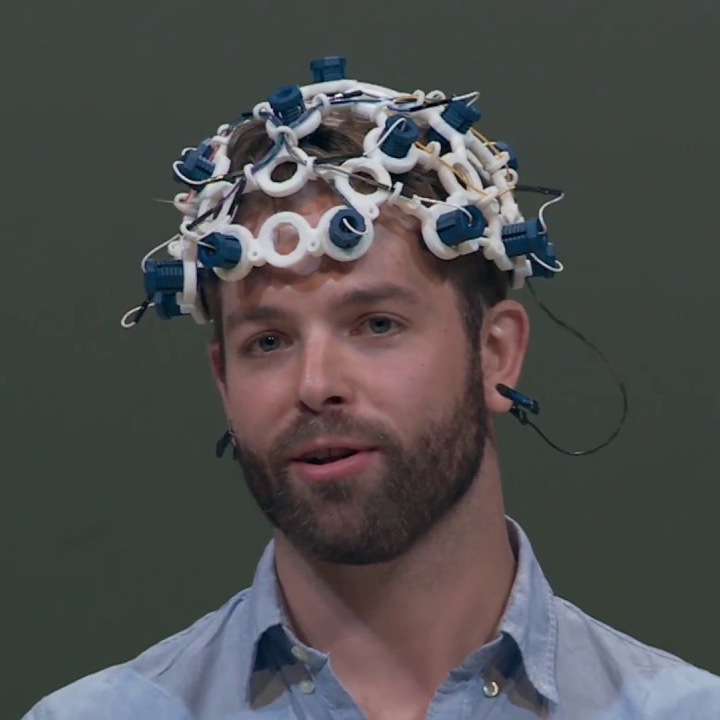
\includegraphics[width=\linewidth]{openbci.jpeg}
  \caption{OpenBCI's EEG \\ device \citep{be_superhvman_conor_2017}}
  \label{fig:openbci}
  \endminipage\hfill
  \minipage{0.32\textwidth}
  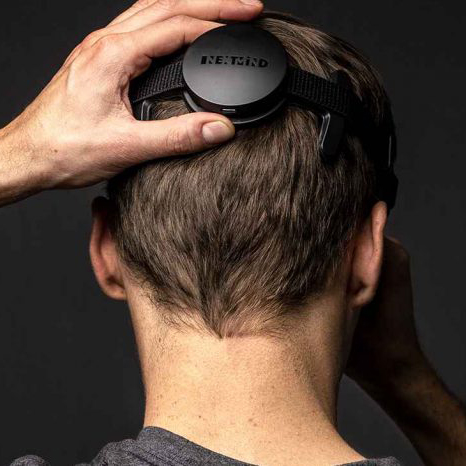
\includegraphics[width=\linewidth]{nextmind.jpeg}
  \caption{NextMind's BCI \\ device \citep{louise_neurotechnology_2019}}
  \label{fig:nextmind}
  \endminipage\hfill
  \minipage{0.32\textwidth}%
  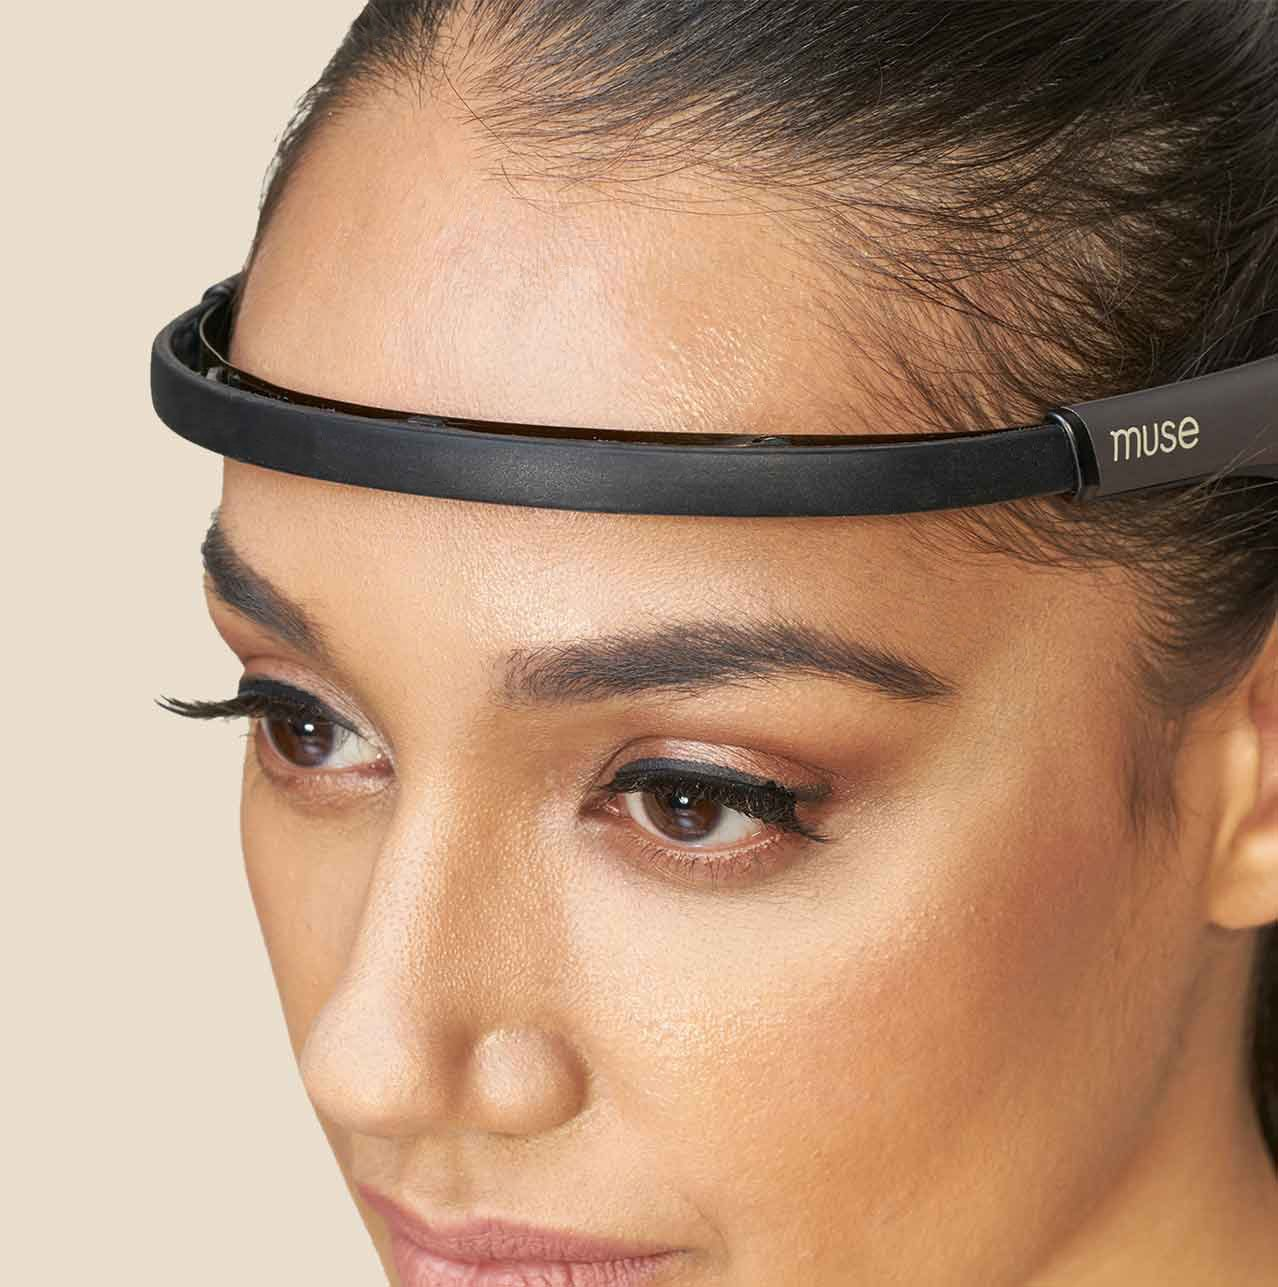
\includegraphics[width=\linewidth]{muse.jpeg}
  \caption{Muse's meditation \\ headband \citep{muse_muse_nodate}}
  \label{fig:muse}
  \endminipage
\end{figure}

A rather closed and specific BCI is, for example, the EEG headband by Muse. Its purpose is to measure meditation and sleep. They also offer an end-user app to help people better understand their meditation and sleep and how to improve them. The Muse headband is not unidirectional BCI per se, as there is also biofeedback based on neural signals, but the important difference between Muse and e.g. OpenBCI is that they abstract away the neurotechnology. Users don't need to know anything about neuroscience, neurotechnology or the interpretation and classification of brain data to get useful functionality for their use case. They also do not need to understand the software system's underlying architecture. The only thing they need to know is how to pair the device with their smartphone via Bluetooth.

Aside from full-stack BCI solutions, where a company provides a complete BCI solution including hardware and software, there are also companies that focus solely on the software aspect of neural data. Neuromore, a company based in Florida and Germany that provides a software platform for everything related to neural signal processing and BCI, is one example. The company is hardware agnostic, which means you can plug any hardware or sensor into your computer and connect it to the Neuromore Studio software. Neuromore Studio is free and open-source software that runs locally on a variety of platforms, including Windows and macOS. It provides a variety of drag-and-drop interfaces for creating and managing signal processing pipelines, even including machine learning classifiers. For example, you can transform EEG data to extract band power and create triggers based on band power selection, and generate conditional outputs for a game to e.g. move a character.

\begin{figure}[ht]
  \centering
  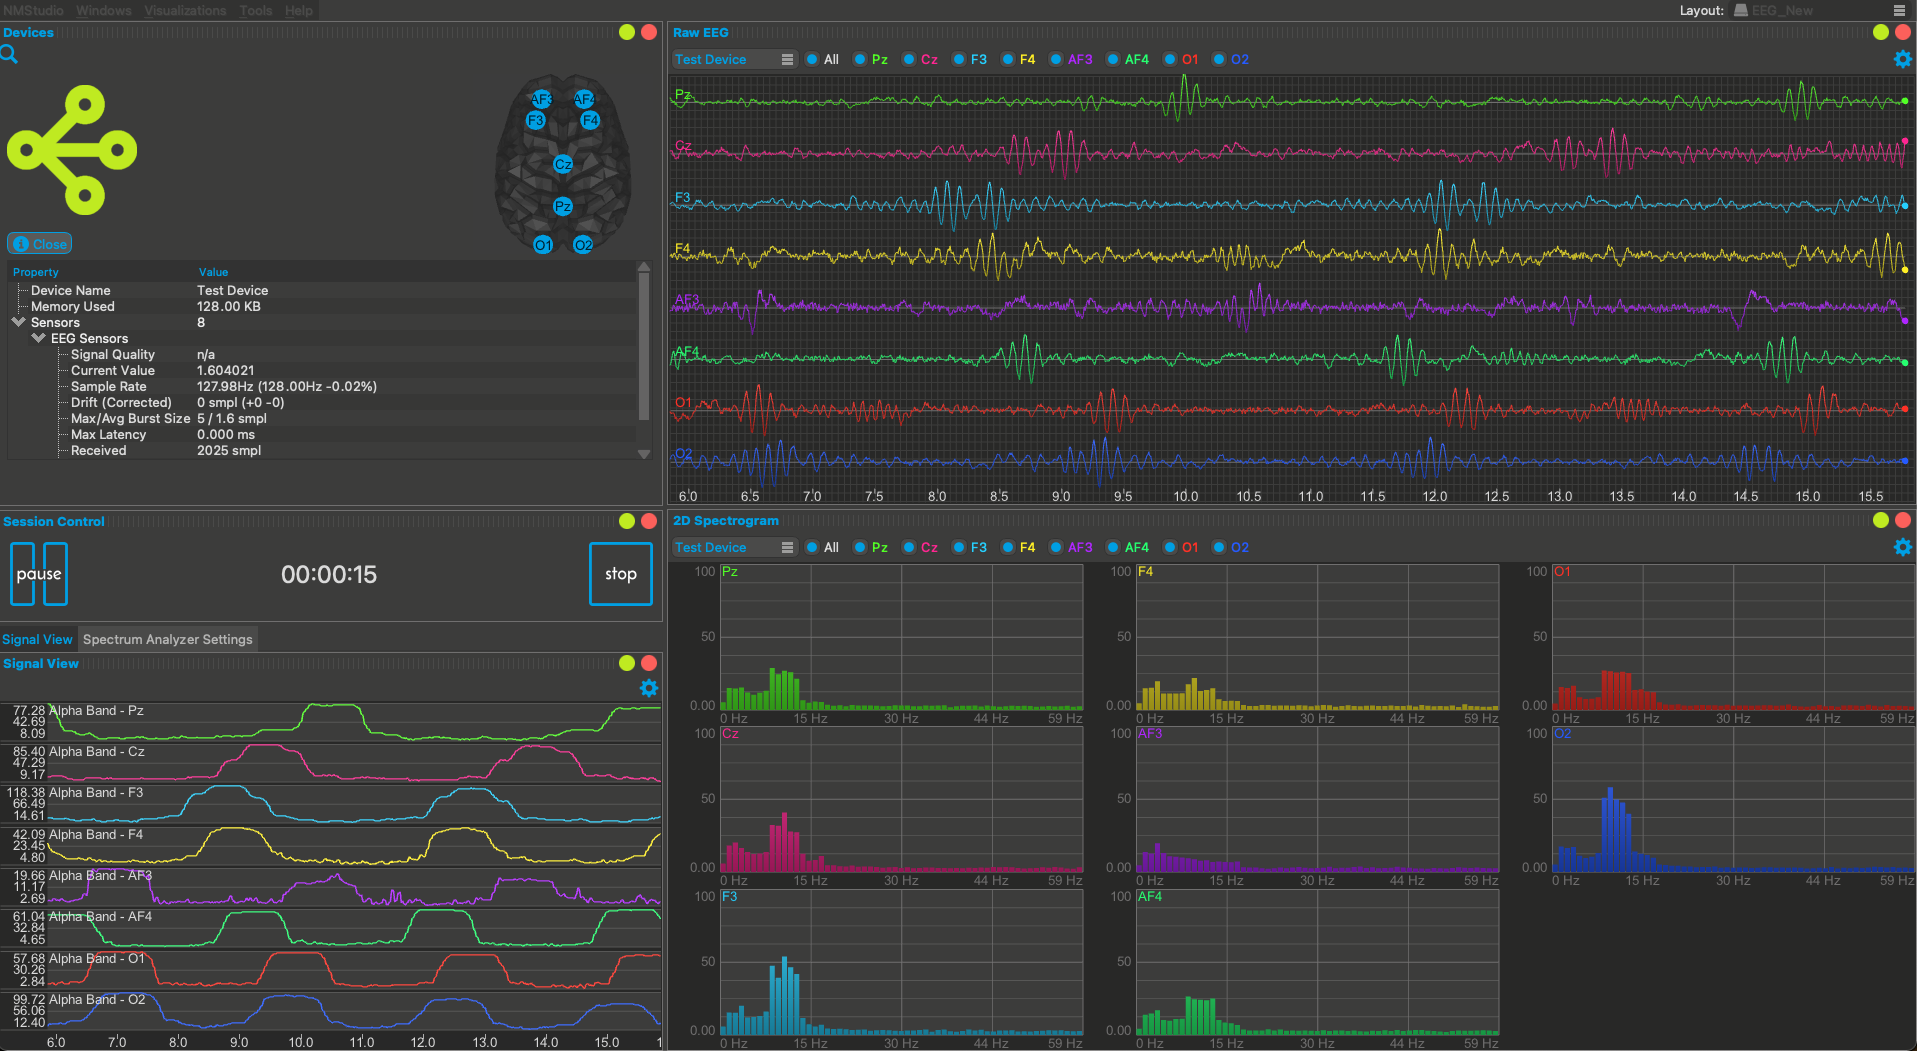
\includegraphics[width=\linewidth]{neuromore.png}
  \caption{Screenshot of the Neuromore Studio software \citep{neuromore_neuromore_nodate}.}
  \label{fig:neuromore}
\end{figure}

The author attempts to differentiate the offerings of the consumer-oriented BCIs mentioned: They either provide the hardware (with software that at least connects to the device) but are then more broadly applicable to use cases not defined by the company behind the BCI, such as OpenBCI, or they are application-specific in terms of both the software and the hardware, such as the Muse headband\footnote{Third-party developers have reverse engineered the Bluetooth features to access Muse's raw EEG data and turn it into a general-purpose device.}.

Despite the fact that this paper focuses on consumer-oriented BCIs, the applications of various BCI offerings can still be distinguished based on whether they are more consumer-oriented or research-oriented, such as the distinction between e.g. NeuroSky\footnote{NeuroSky website: https://neurosky.com} for hobbyists and Emotiv's\footnote{Emotiv website: https://emotiv.com} EEG systems, which are more research-oriented.

However, both NeuroSky and Emotiv provide a research version as well as a consumer or enterprise version of their software and hardware, aiming for general-purpose applicability across customer segments and use cases.

Other considerations include whether the applications are rather steady state evoked such as based on a frequency of noise laid on top of virtual objects to detect which object the person is looking at (e.g. as NextMind is doing), or whether they track the totality of mental states without evoking neural signals with external stimuli, such as in tracking sleep or concentration levels, both of which arise primarily evoked from inside the mind. This distinction can be made as passive, active or reactive BCI, as \citeauthor{alimardani_passive_2020} coined in their work on passive BCIs \citep{alimardani_passive_2020}. However, we do not want to include this dimension because it would introduce unnecessary and additional complexities that are more related to the application layer of BCI software.

\begin{figure}[!ht]
  \centering
  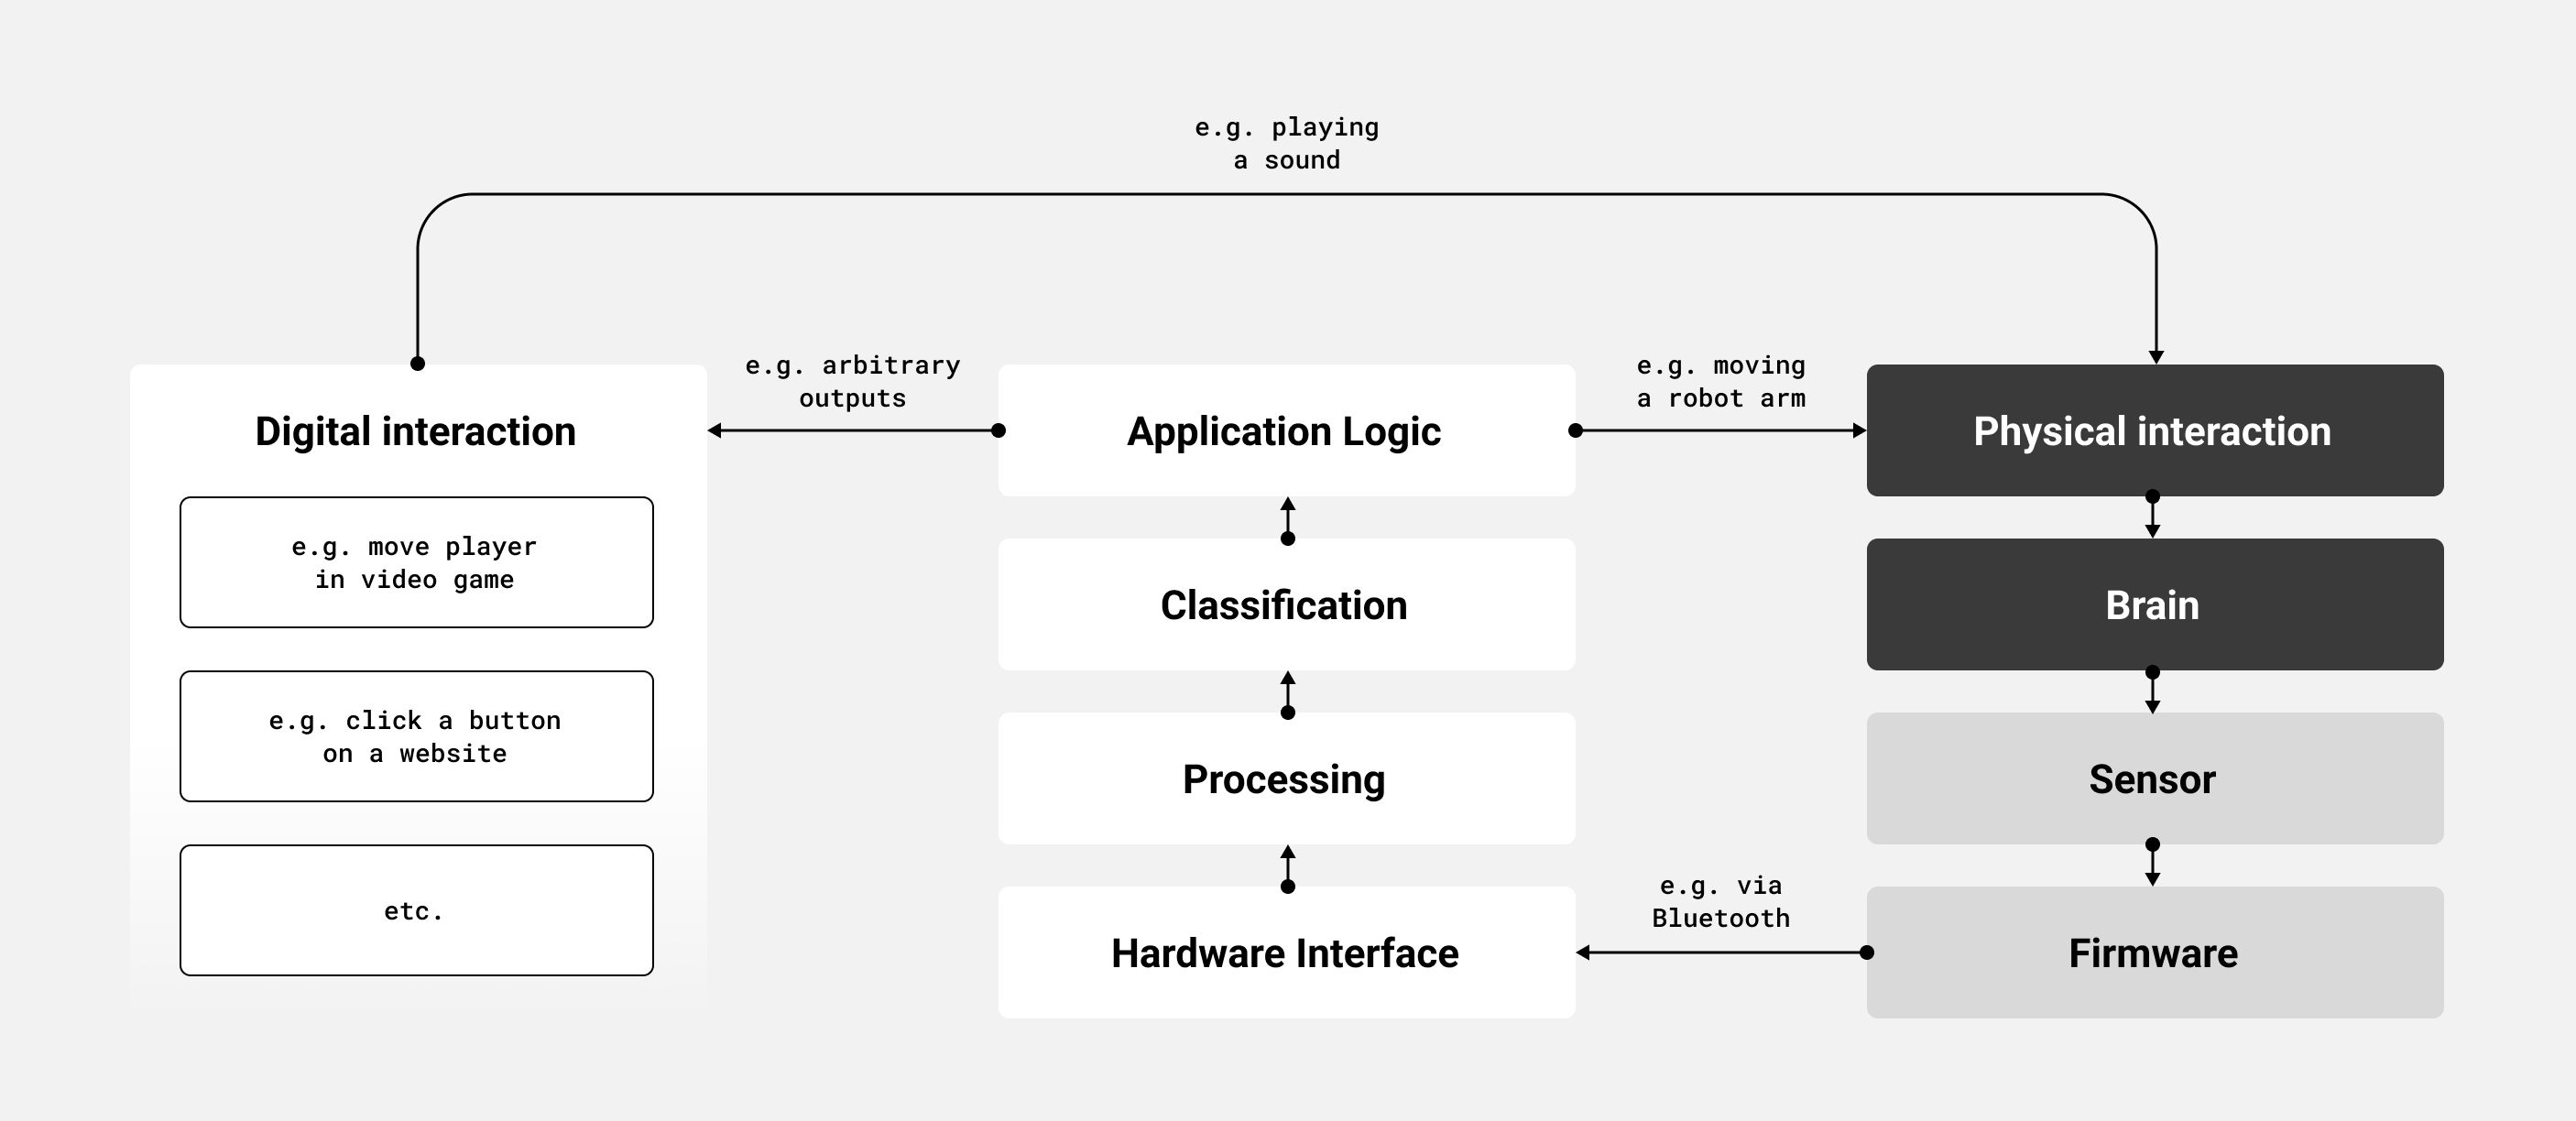
\includegraphics[width=\linewidth]{bci-components.png}
  \caption{Architectural overview of BCI components including a bidirectionality due to neurofeedback in form of e.g. playing a sound in a certain frequency to enable SSVEP (own representation, 2022).}
  \label{fig:bci-components}
\end{figure}

As shown on \autoref{fig:bci-components} there are two main components of a BCI: the hardware and the software. Next to the hardware, there is also the physical part of it, e.g. the brain and a physical interaction counterpart in form of e.g. a robot arm\footnote{Some people call this a brain-machine interface rather than a brain-computer interface because you interface with a machine rather than a computer.}. The software is the part that is responsible for the actual processing of the data, e.g. extracting the relevant information from the raw data and turning it into a meaningful output that the application layer can use. The application layer interacts then with a physical or digital counterpart to e.g. move a player in a game or turn start playing sound on the computer via its speakers.

\subsection{Unobtrusive hardware and software}
\label{chapter2-unobtrusive-hardware-and-software}

Another essential aspect of BCI the unobtrusiveness of hardware and software. Unobtrusiveness in hardware means that it's either not visible at all because it's e.g. implanted sensors under the skull or because it is in a form factor that is socially established already, such as e.g. in a pair of glasses or earphones. On \autoref{fig:unobstrusive-hardware} you can see the prototype of the in-ear EEG hardware from IDUN Technologies that measures the brain activity of a person inside the ear canal. Next to it on \autoref{fig:obstrusive-hardware} is the Neurosity device that measures the brain activity on top of the head, which doesn't resemble a socially established form factor. What's described as socially established and accepted really depends on society and the context, because one could e.g. say that a Neurosity device under a hat is more accepted while talking to a friend compared to having a pair of earphones on you. Nonetheless, if e.g. in-ear EEG technology goes more into the direction of discreetness such as hearing aids then it is more unobtrusive and socially accepted.

\begin{figure}[!htb]
  \minipage{0.49\textwidth}
  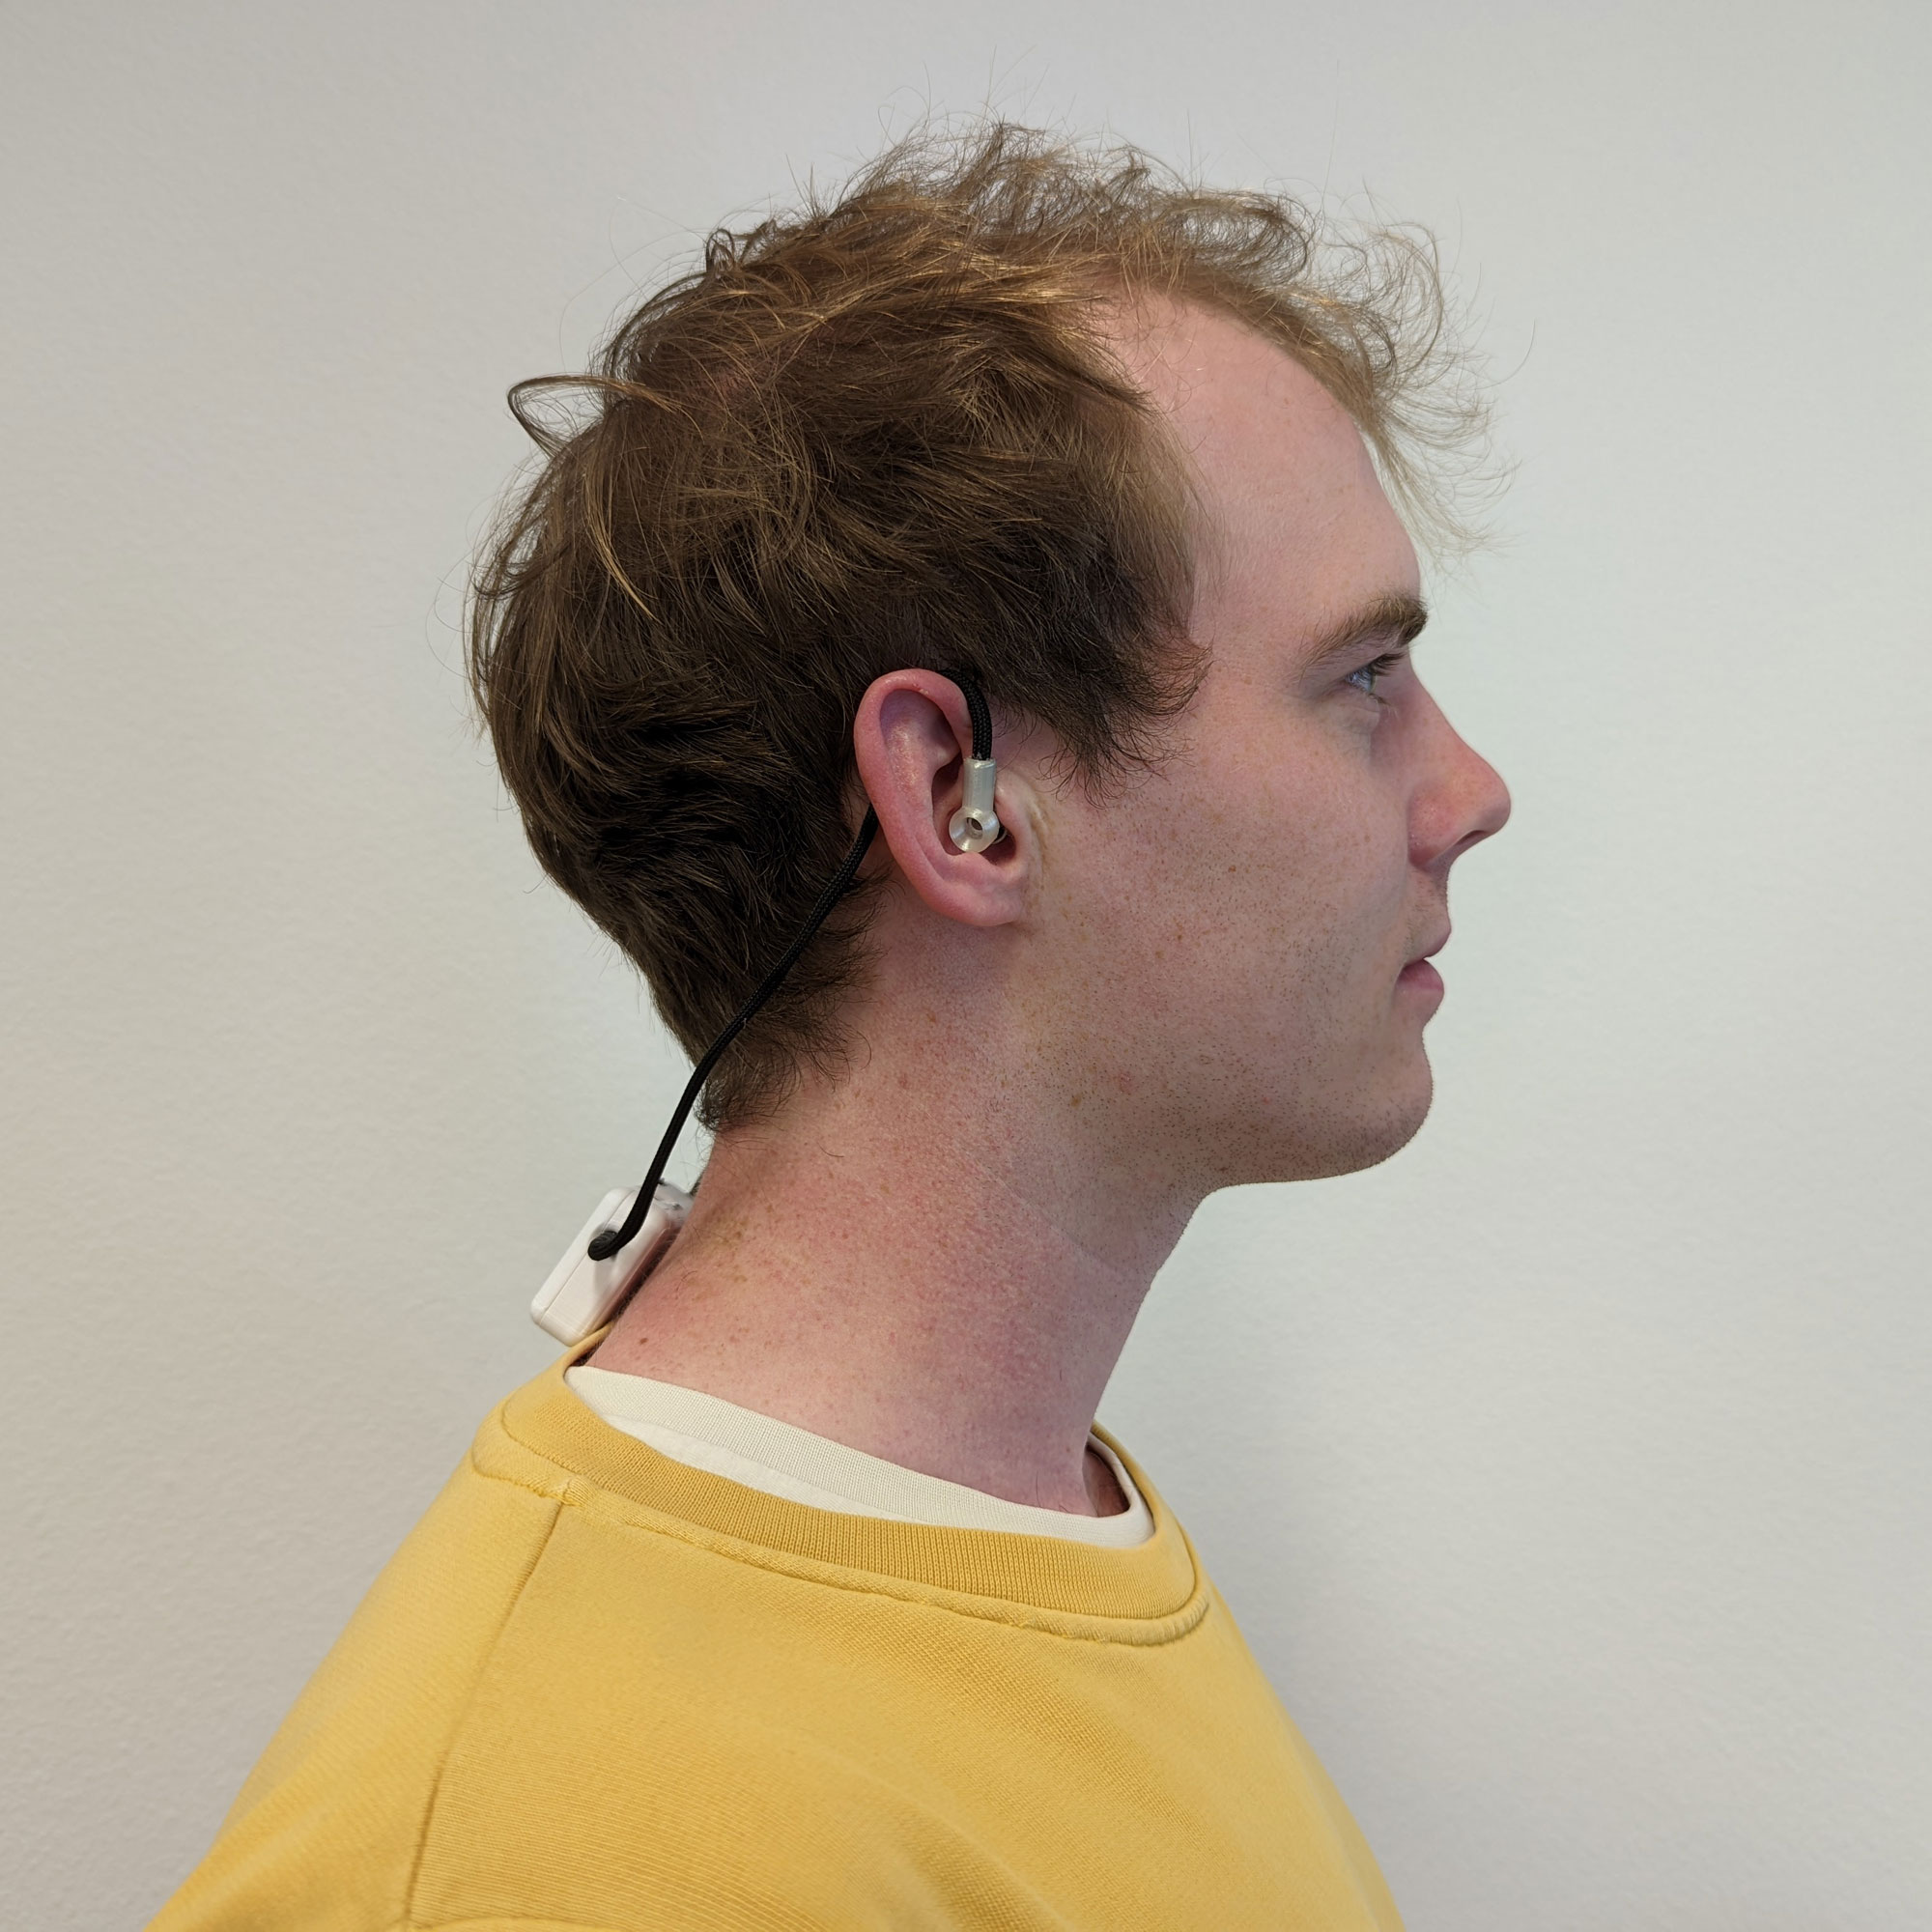
\includegraphics[width=\linewidth]{unobtrusive.jpg}
  \caption{IDUN Guardian hardware, \\ unobtrusive BCI (own representation, 2022).}
  \label{fig:unobstrusive-hardware}
  \endminipage\hfill
  \minipage{0.49\textwidth}
  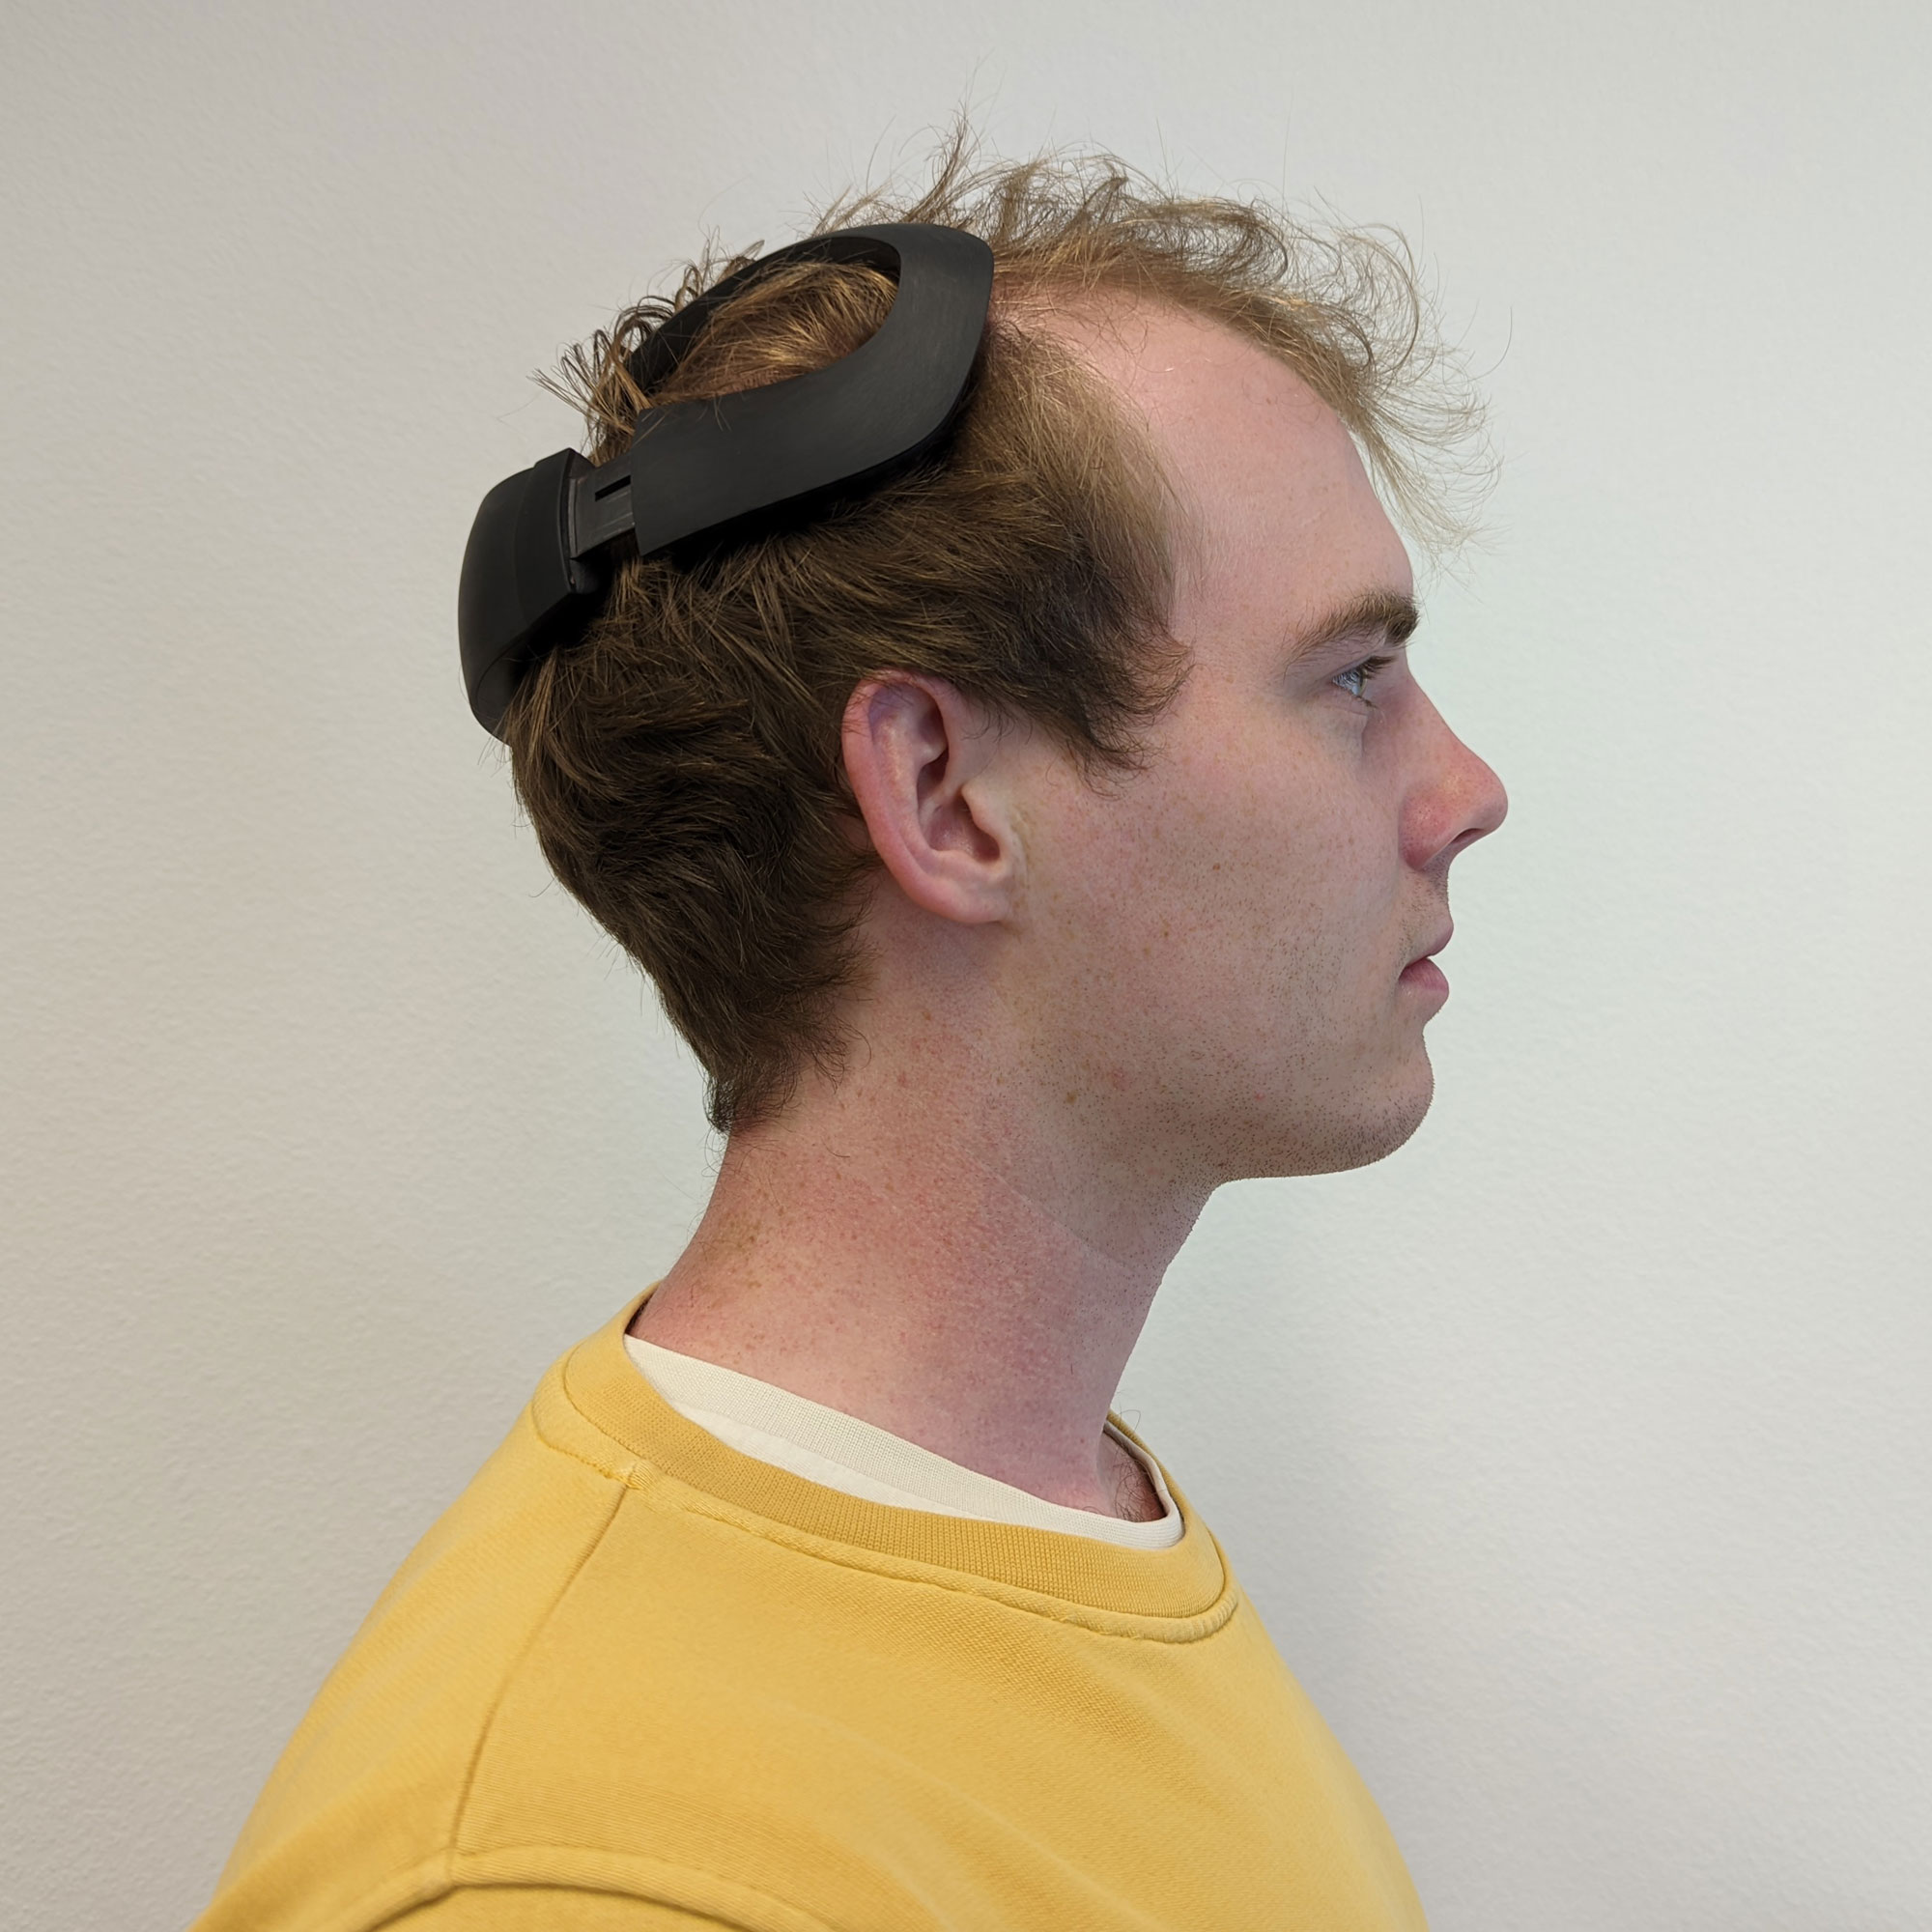
\includegraphics[width=\linewidth]{obtrusive.jpg}
  \caption{Neurosity Notion hardware, \\ obtrusive BCI (own representation, 2022).}
  \label{fig:obstrusive-hardware}
  \endminipage\hfill
\end{figure}

Adding brain sensing sensors to a form factor e.g. in wearables that are established is a possibility for BCI hardware to go to the masses, but introducing a completely new wearable form factor like e.g. Neurosity tries to do, can be looked at very critical for mass adoption. One also has to consider the implications different form factors bring with them e.g. the ability to move the device and therefore creating motion artefacts in the signals or the location of the sensors based on the form factor. The ear canal is e.g. optimal for the hearing-related part of the brain but not so optimal for the visual cortex which is on the back on the head. But this is a topic that is not covered in this thesis.

Next to that comes the mobility. If a device might be unobtrusive in the form factor itself but needs cables to be connected to the computer, then the mass adoption usually seems harder. An example of this comes from another industry: VR. The most sold and mass-market VR headset to date is the Meta Quest 2, next to the USPs in the software, one notable compared to others is that it was a mobile and all-in-one device without the need of external motion capture sensors or cables.

When talking about the unobtrusiveness of software it might not be as straightforward as it is with hardware. What the author understands under unobtrusive software is the abstraction of underlying software that runs logic to make the desired thing work. As an example of obtrusive software: in order to use a HP printer with your Android mobile phone, you need to download the HP Printer app and a companion app which acts as a driver for the printer. Afterwards, you can start printing documents to the printer via Wifi. In this case, the user needs to understand some of the underlying technical architecture to make it work, rather than just selecting the printer and then print. Unobtrusive software is e.g. when you have a new computer mouse, you plug it in and it just works.

Coming to BCI software unobtrusive software means that you can connect your hardware to your computer or smartphone and use it without any additional software, such as moving the cursor, or clicking on buttons. This is currently not possible with the current state of the art, but it is possible with some additional software. To give you an example of e.g. choosing an OpenBCI device, you need to open the GUI app, connect the hardware, start a recording session, output the stream as an lab streaming-layer (LSL), connect to that stream from e.g. Neuromore Studio, let the data run through a classification pipeline to then connect the outputs of Neuromore to a video game via a SDK inside the engine itself to then have controls for the video game. It should become pretty clear that this cannot be considered unobtrusive software.

Of course there are examples of BCI software that is as unobtrusive as possible, such as e.g. the  app.

\subsection{Cloud paradigm-shift}
\label{chapter2-cloud-paradigm-shift}

Lorem ipsum dolor sit amet.

% Mention Neuropype

% Challenges and requirements of going with a cloud, API and SDK (privacy, security, IP, performance, scaling etc.)

\section{Web-first approach to software}
\label{chapter2-web-first-approach-to-software}

% What production-grade software separates from others
% Use The Twelve Factors as a reference

% \subsection{Modern web APIs for BCI}
% \label{chapter2-modern-web-apis-for-bcis}

% Examples of BCI data going through web stacks, how to make it work (paper from Stegman)
% Use this as well https://urish.medium.com/reactive-brain-waves-af07864bb7d4

% \subsection{3D applications in the browser}
% \label{chapter2-3d-applications-in-the-browser}

% Current state of 3D on the web (WebGPU, pixel streaming, declarative graphics components, WebAssembly (and Rust), etc.)

\section{Web-based AR and VR}
\label{chapter2-web-based-ar-and-vr}

% Current state of VR and AR applications (Meta Quest, Snapchat, ARKit, etc.)

\section{Neural/cloud interfacing definition}
\label{chapter2-neural-cloud-interfacing-definition}

\begin{figure}[ht]
  \centering
  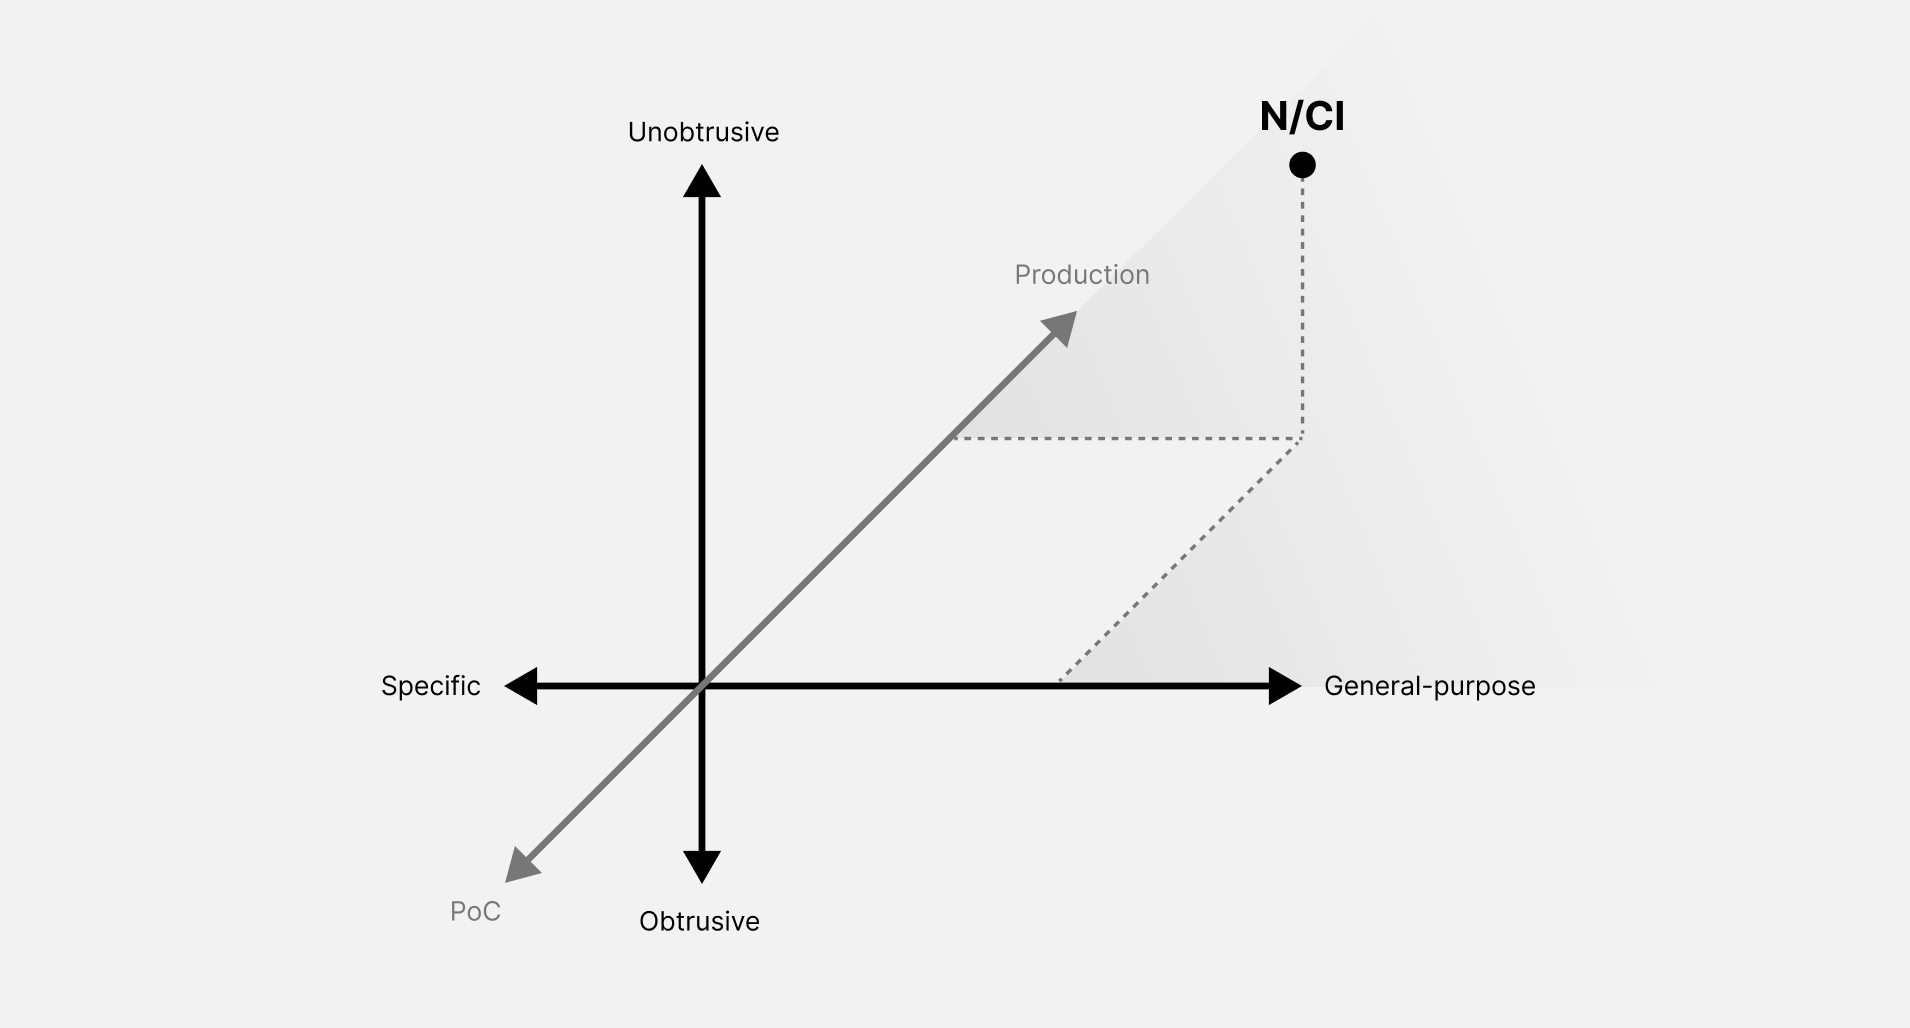
\includegraphics[width=\linewidth]{nci-definition.png}
  \caption{Visualisation of the three-dimensionality of the term neural/cloud interface (own representation, 2022).}
  \label{fig:nci-definition}
\end{figure}

% General definition of a N/CI
% General challenges of a N/CI

% Difference between existing software systems that come close to a N/CI
% Opt-in is based on ourselves rather than an account
% Unobtrusiveness of the software (SDK), down to the OS layer (give example of the printer scenario from Auriel)
% Create another list with the challenges of a N/CI and use them for the solutions in the methodologies and implementation sections

% Akademischer Hintergrund: Vorbilder, Referenzmaterial, Eingrenzung und vertiefte Begründung der Zielformulierung. Grundlagenforschung im Bereich vergleichbarer Medienprodukte. Kenntnis der fachspezifischen Theorien und Techniken. Hier muss umfassende Fach- und Handwerkskenntnis gezeigt werden. Es sollen möglichst viele Informationen verwendet werden, die helfen sollen Entscheidungen für die Erstellung des eigenen Medienprodukts zu treffen und Vorgehensweisen beim Entstehungsprozess des eigenen Medienprodukts zu begründen. Ebenso soll begründet werden, inwiefern die verwendeten Quellen für die Zielsetzung und deren Umsetzung geeignet sind.

\nomenclature[nlu\]{NLU}{Natural language understanding}
\nomenclature[agi\]{AGI}{Artificial general intelligence}
\nomenclature[fmri]{fMRI}{Functional magnetic resonance imaging}
\nomenclature[tdfnirs]{TD-fNIRS}{Time-domain functional near-infrared spectroscopy}
\nomenclature[gui]{GUI}{Graphical user interface}
\nomenclature[ssvep]{SSVEP}{Steady-state visual evoked potential}
\nomenclature[lsl]{LSL}{Lab streaming layer}
